\documentclass{report}

\usepackage{subcaption} % package for subfigures
\usepackage{hyperref}  % package for linking figures etc
\usepackage{enumitem}  % package for description with bullets
\usepackage{graphicx}  % package for importing images
\usepackage{mathtools} % package for math equation
\usepackage{mathrsfs}  % package for math font
\usepackage{indentfirst} % package for getting ident after section or paragraph
\usepackage[export]{adjustbox}
% \usepackage{amsmath}

\setlength{\parindent}{2em} % how much indent to use when we start a paragraph

\graphicspath{ {./theory/figures/} }       % path for images

\begin{document}

\chapter{Connecting Tubes}
\section{Description}
After getting TOIs for each video segment, it is time to connect them. That's because most actions in videos lasts more that 16 frames.
This means that, in overlaping video clips, there will be consequentive TOIs that represent the entire action. So, it is essential to create
an algorithm for finding and connecting these TOIs.
\subsection{First approach: combine overlap and actioness}
Our algorithm is inspired by \cite{DBLP:journals/corr/HouCS17}, which calculates all possible sequences of ToIs. In order find the best candidates, it uses a score which tells us how likely a sequence of TOIs is  to contain an action. This score is a combination of 2 metrics:
\begin{description}
\item[ Actioness,  ] which is the TOI's possibility to contain an action. This score is produced by TPN's scoring layers.
\item [ TOIs' overlapping, ] which is the IoU of the last frames of the first TOI and the first frames of the second TOI.
\end{description}

The above scoring policy can be described by the following formula:
\[ S = \frac{1}{m} \sum_ {i=1}^{m} Actioness_i + \frac{1}{m-1} \sum_{j=1}^{m-1} Overlap_{j,j+1} \]

For every possible combination of TOIs we calculate their score as show in figure \ref{fig:connection_algo}.
The above approach, however, needs too much memory for all needed calculations, so a memory usage  problem is
appeared. The reason is, for every new video segments we propose \textit{k TOIs} (16 during training and 150 during validation).
As a result, for a small video seperated in  \textbf{10 segments}, we need to calculate 
\textbf{  150\textsuperscript{10} scores} during validation stage. \par

\begin{figure}[h]
  \centering
  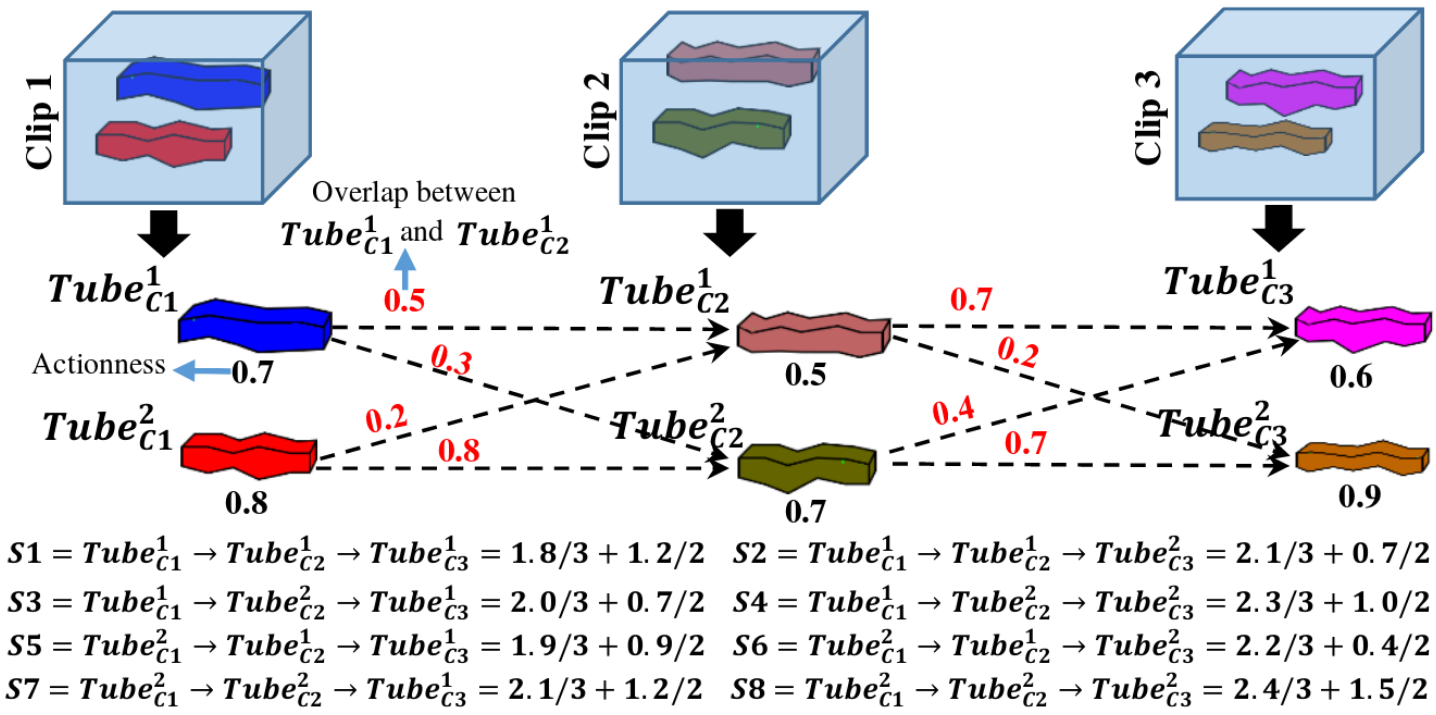
\includegraphics[scale=0.225]{connection_algo}
  \caption{An example of calculating connection score for 3 random TOIs}
  \label{fig:connection_algo}
\end{figure}

In order to deal with this problem, we create a greedy algorithm in order to find the candidates tubes. Inituitively, this algorithm after
a new video segment keeps tubes with score higher than a threshold, and deletes the rest.
So, we don't need to calculate combinations with very low score. This algorithm is described below:
\begin{enumerate}
\item Firstly, initialize empty lists for the final tubes, their scores, active tubes, their overlapping sum and actioness sum where:
  \begin{itemize}
  \item Final tubes list contains all tubes which are the most possible to contain an action, and their score list contains their
    corresponding scores.
  \item Active tubes list contains all tubes that will be match with the new TOIs. Their overlapping sum list and actioness sum list
    contain their sums in order to avoid calculating then for each loop. 
  \end{itemize}
Also, we initialize threshold equal to 0.5 .
\item For the first video segment, we add all the TOIs to both active tubes and final tubes. Their scores are only their actioness because
  there are no tubes for calculating their overlapping score. So, we set their overlaping sum equal to 0.
\item For each next video, firstly we calculate their overlapping score with each active tube. Then, we empty active tubes, overlapping
  sum and actioness score lists.  For each new tube that has score higher than the threshold we add to final tubes and to active tubes.
\item If the number of active tubes is higher than a threshold (1000 in our situation), we set the threshold equal to the score of
  the 100th higher score. On top of that, we update the final tubes list, removing all tubes that have score lower than the threshold.
\item After that, we add in active tubes, the current video segment's proposed TOIs. Also their actioness scores in actioness sum list and
  zero values in corrensponding positions in overlaps sum list (such as in the 1st step).
\item We repeat the previous 3 steps until there is no video segment left.
\end{enumerate}
% We implement this algorithm using CUDA language for counting the scores. In \cite{DBLP:journals/corr/HouCS17}, they use temporal \textit{stride = sample duration} during testing. We want 
\section{Some results}

In order to validate our algorithm, we firstly experiment in JHMDB dataset's videos in order to define the best overlapping policy and
the video overlapping step. We consider as positive if there is at least 1 video tube which overlaps with the groundtruth video tube
over a predefined threshold.  These thresholds are 0.5, 0.4 and 0.3. 

\paragraph{sample duration = 16} At first we use as sample duration = 16 and video step = 8. As overlapping frames we count frames
\textit{(8...15)} so we have \#8 frames. Also, we use only \#4 frames with combinations \textit{(8...11), (10...13) and (12...15)} and 
\#2 frames with combinations \textit{(8,9), (10,11), (12,13), and (14,15)}. Then, we set video step = 12. In this case, for \#4 frames, we
only have the combination \textit{(12...15)}, for \#2 frames we have \textit{(12,13), (13,14) and (14,15)}. Finally, we set video step = 14
with combinations, for \#2 frames \textit{(14,15)}, for \#1 frame \textit{(14) and (15)}; and for video step = 15, the only combination in
frame \textit{(15)}.

TODO table with results.

As we can see in the above table, in validation step, the best result is in combination for step = 15 and overlapping frames only frame \#15.

\paragraph{sample duration = 8}

\paragraph{sample duration = 4}


 
\subsection{UCF dataset}


\subsection{Second approach: use progression and progress rate}
As we saw before, our first connecting algorithm doesn't have very good recall results. So, we created another algorithm which is base in \cite{}. This
algorithm introduces two 2 metrics according to \cite{}:

% TODO add more description
\begin{description}
\item[ Progression,  ] which describes the probability of a specific action being performed in the TOI. 
% We add this factor because we have noticed that actioness
%   is tolerant to false positives. Progression is mainly a rescoring mechanism for each class.

\item [ Progress rate, ] which is defined as the progress proportion that each class has been perfomed.
  
\end{description}

So, each action tube is describes as a set of TOIs
\[  T = {\{ {\bf t}_i^{(k)} | {\bf t}_i^{(k)} = ( t_i^{(k)}, s_i^{(k)}, r_i^{(k)} ) \}}_{i=1:n^{(k)},k=1:K} \]
where $ t_i^{(k)} $ contains TOI's spatiotemporal information, $ s_i^{(k)} $ its confidence score and $ r_i^{(k)} $ its progress rate.

In this approach, each class is handled seperately, so we discuss action tube generation for one class only. In order to link 2 TOIs, for
a video with N video segments, the following steps are applied:
\begin{enumerate}
\item For the first video segment (k = 1), initialize an array with the M best scoring TOIs, which will be considered as active action tubes ( AT ).
  Correspondly, initialize an array with M progress rates  and M confidence scores.
\item For k = 2:N, execute (a) to (c) steps:
  \begin{enumerate}
  \item Calculate overlaps between $ AT^{(k)} $ and $ TOIs^{(k)}. $
  \item Connect all tubes which satisfy the following criterions:
    \begin{enumerate}
    \item $ overlap score(at_i^{(k)},t_j^{(k)})   < \theta, 
      at  \varepsilon AT^{(k)}, t \varepsilon TOIs^{(k)}  $
    \item $r(at_i^{(k)}) < r(t_j^{(k)}) $ or 
      $r(t_i^{(k)}) - r(at_i{(k)}) < \lambda $
    \end{enumerate}
    
  \item For all new tubes update confidence score and progress rate as follows:
    \begin{description}
    \item New cofidence score is the average score of all connected TOIs:
      \[  s_z^{(k+1)} = \frac {1} {n} \sum_{n=0}^{k} s_i^{(n)}\]
    \item New progress rate is the highest progress rate:
      \[r(at_z^{(k+1)} = max(r(at_i^{(k)}), r(t_j^{(k)})) \]
    \end{description}
    % \item If $ progressrate(at_i^{(k)}) < progressrate(t_i^{(k)}) $ then $ progressrate(at_i^{(k+1)}) =
  \item Keep M best scoring action tubes as active tubes and keep K best scoring action tubes for classification.
  \end{enumerate}
  
\end{enumerate}




\end{document}
